%
% tools.tex
%
% Copyright (C) 2019 by Gabriel Mariano Marcelino <gabriel.mm8@gmail.com>.
%
% Relatório 3 do Trabalho Final da Disciplina EEL510265.
%
% This work is licensed under the Creative Commons Attribution-ShareAlike 4.0
% International License. To view a copy of this license,
% visit http://creativecommons.org/licenses/by-sa/4.0/.
%

%
% \brief Tools section.
%
% \author Gabriel Mariano Marcelino <gabriel.mm8@gmail.com>
%
% \version 0.1.0
%
% \date 21/11/2019
%

\section{Ferramentas Utilizadas} \label{sec:tools}

Para o desenvolvimento do projeto, utilizou-se como principal ferramenta o compilador ``gcc'' \cite{gcc} (em sua variante para C++: ``g++'', versão 9.2.1), neste caso para o desenvolvimento geral e específico da variante do \textit{software} que é executada em um microcomputador.

Para a versão do \textit{software} que será embarcada, se utilizará as ferramentas de desenvolvimento da respectiva plataforma, que neste caso são: ST-Link \cite{stlink} (ferramenta para carregar o \textit{firmware} na plataforma alvo), o compilador para a plataforma ARM (``arm-none-eabi-g++'' \cite{gcc_arm}), e a biblioteca para acessar os periféricos da plataforma alvo (``libopencm3'' \cite{libopencm3}).

Além dessas ferramentas de \textit{software}, também está se utilizando o \textit{kit} de desenvolvimento STM32 Discovery \cite{stm32_discovery} e um conversor USB-UART para fazer a leitura das entradas de log do sistema (através de uma porta serial do \textit{kit} de desenvolvimento). Ambos podem ser vistos na \autoref{fig:tools}.

\begin{figure}[!ht]
    \begin{center}
        \subfigure[STM32-F4 Discovery.]{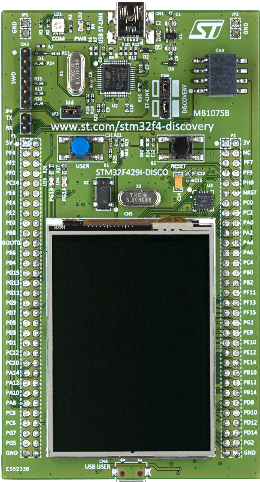
\includegraphics[width=0.2\textwidth]{figures/stm32f4_discovery.jpg}}
        \qquad
        \subfigure[Conversor USB-UART.]{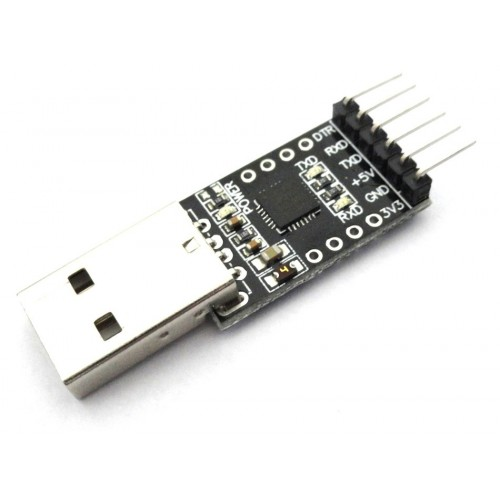
\includegraphics[width=0.35\textwidth]{figures/usb-uart_converter.jpg}}
        \caption{Principais ferramentas físicas utilizadas.}
        \label{fig:tools}
    \end{center}
\end{figure}
